\section{mr::timer Class Reference}
\label{classmr_1_1timer}\index{mr::timer@{mr::timer}}
{\tt \#include $<$mr\-Profile.h$>$}

Inheritance diagram for mr::timer::\begin{figure}[H]
\begin{center}
\leavevmode
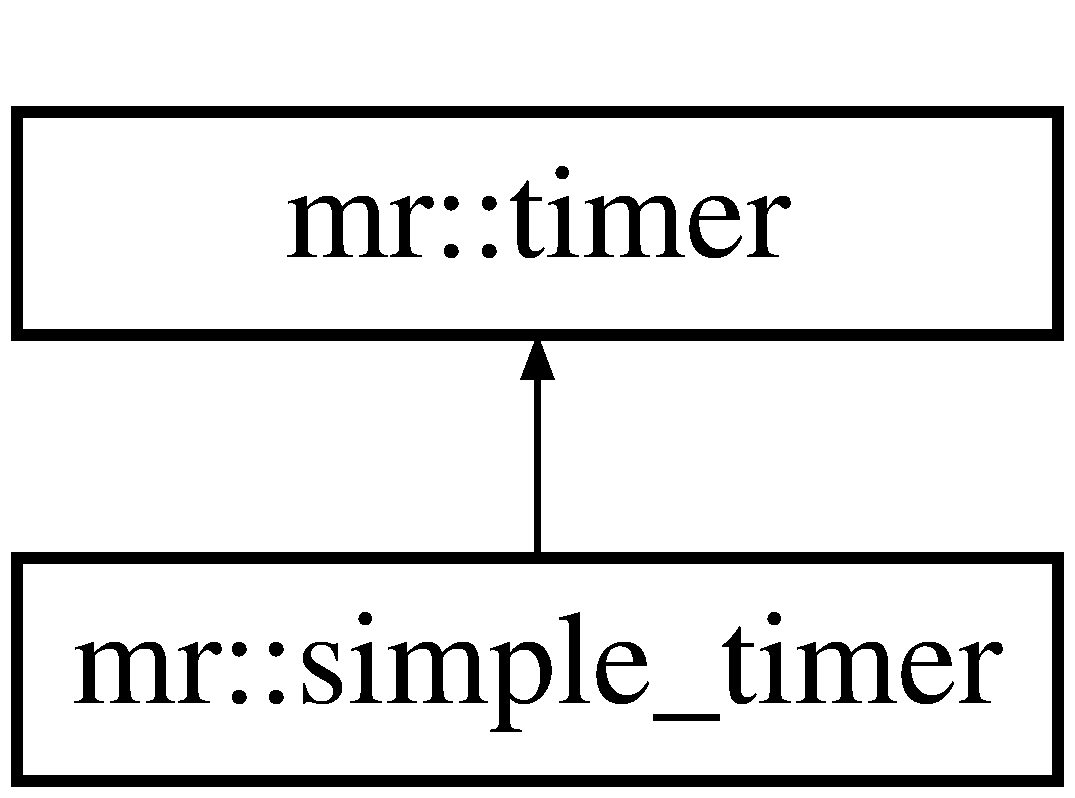
\includegraphics[height=2cm]{classmr_1_1timer}
\end{center}
\end{figure}
\subsection*{Public Member Functions}
\begin{CompactItemize}
\item 
{\bf timer} (mi\-Uint l=0)
\item 
{\bf timer} (const {\bf timer} \&b)
\item 
{\bf $\sim$timer} ()
\item 
void {\bf print} ()
\item 
void {\bf start} ()
\item 
void {\bf stop} ()
\item 
bool {\bf operator$>$} (const {\bf timer} \&b) const 
\item 
bool {\bf operator$<$} (const {\bf timer} \&b) const 
\item 
{\bf timer} \& {\bf operator+=} (const {\bf timer} \&b)
\item 
{\bf timer} \& {\bf operator-=} (const {\bf timer} \&b)
\end{CompactItemize}


\subsection{Detailed Description}
Very simple class/macro for profiling stuff... Just use it like:



\footnotesize\begin{verbatim}       mr::timer t1;
       // ... stuff to profile goes here...
       t1.stop();
   
       mr::timer t2;
       // ... stuff to profile goes here...
       t2.stop();
   
       if ( t1 < t2 ) mi_info("t1 is faster");
       else mi_info("t2 is faster");
\end{verbatim}
\normalsize




\subsection{Constructor \& Destructor Documentation}
\index{mr::timer@{mr::timer}!timer@{timer}}
\index{timer@{timer}!mr::timer@{mr::timer}}
\subsubsection{\setlength{\rightskip}{0pt plus 5cm}mr::timer::timer (mi\-Uint {\em l} = 0)\hspace{0.3cm}{\tt  [inline]}}\label{classmr_1_1timer_a0}


\index{mr::timer@{mr::timer}!timer@{timer}}
\index{timer@{timer}!mr::timer@{mr::timer}}
\subsubsection{\setlength{\rightskip}{0pt plus 5cm}mr::timer::timer (const {\bf timer} \& {\em b})\hspace{0.3cm}{\tt  [inline]}}\label{classmr_1_1timer_a1}


\index{mr::timer@{mr::timer}!~timer@{$\sim$timer}}
\index{~timer@{$\sim$timer}!mr::timer@{mr::timer}}
\subsubsection{\setlength{\rightskip}{0pt plus 5cm}mr::timer::$\sim${\bf timer} ()\hspace{0.3cm}{\tt  [inline]}}\label{classmr_1_1timer_a2}




\subsection{Member Function Documentation}
\index{mr::timer@{mr::timer}!operator+=@{operator+=}}
\index{operator+=@{operator+=}!mr::timer@{mr::timer}}
\subsubsection{\setlength{\rightskip}{0pt plus 5cm}{\bf timer}\& mr::timer::operator+= (const {\bf timer} \& {\em b})\hspace{0.3cm}{\tt  [inline]}}\label{classmr_1_1timer_a8}


\index{mr::timer@{mr::timer}!operator-=@{operator-=}}
\index{operator-=@{operator-=}!mr::timer@{mr::timer}}
\subsubsection{\setlength{\rightskip}{0pt plus 5cm}{\bf timer}\& mr::timer::operator-= (const {\bf timer} \& {\em b})\hspace{0.3cm}{\tt  [inline]}}\label{classmr_1_1timer_a9}


\index{mr::timer@{mr::timer}!operator<@{operator$<$}}
\index{operator<@{operator$<$}!mr::timer@{mr::timer}}
\subsubsection{\setlength{\rightskip}{0pt plus 5cm}bool mr::timer::operator$<$ (const {\bf timer} \& {\em b}) const\hspace{0.3cm}{\tt  [inline]}}\label{classmr_1_1timer_a7}


\index{mr::timer@{mr::timer}!operator>@{operator$>$}}
\index{operator>@{operator$>$}!mr::timer@{mr::timer}}
\subsubsection{\setlength{\rightskip}{0pt plus 5cm}bool mr::timer::operator$>$ (const {\bf timer} \& {\em b}) const\hspace{0.3cm}{\tt  [inline]}}\label{classmr_1_1timer_a6}


\index{mr::timer@{mr::timer}!print@{print}}
\index{print@{print}!mr::timer@{mr::timer}}
\subsubsection{\setlength{\rightskip}{0pt plus 5cm}void mr::timer::print ()\hspace{0.3cm}{\tt  [inline]}}\label{classmr_1_1timer_a3}


\index{mr::timer@{mr::timer}!start@{start}}
\index{start@{start}!mr::timer@{mr::timer}}
\subsubsection{\setlength{\rightskip}{0pt plus 5cm}void mr::timer::start ()\hspace{0.3cm}{\tt  [inline]}}\label{classmr_1_1timer_a4}


\index{mr::timer@{mr::timer}!stop@{stop}}
\index{stop@{stop}!mr::timer@{mr::timer}}
\subsubsection{\setlength{\rightskip}{0pt plus 5cm}void mr::timer::stop ()\hspace{0.3cm}{\tt  [inline]}}\label{classmr_1_1timer_a5}




The documentation for this class was generated from the following file:\begin{CompactItemize}
\item 
{\bf mr\-Profile.h}\end{CompactItemize}
